% =====================================================================
\chapter{Part A: Simulation Results}
\label{ch:parta-results}
\thispagestyle{plain}
% =====================================================================

\section{Introduction}

This chapter evaluates the Part~A methods. Section~\ref{sec:ra-comp} reports compression ratio, error, encode time and SNR robustness of CSEE and RAS-BFP against O-RAN BFP and truncated SVD. Section~\ref{sec:ra-bench} reports the eight-method inversion screening benchmark. Section~\ref{sec:ra-rmtws} evaluates RMT-WS on realistic complex precoding channels: spectral-interval coverage, cold-start cost, tracking across user speeds, the Doppler law and low-precision robustness. Section~\ref{sec:ra-ru} quantifies the fronthaul saving of RU-side precoding. The simulation parameters are listed in Table~\ref{tab:a-params}.

\begin{table}[H]
\caption{Part~A simulation parameters.}
\label{tab:a-params}
\centering\small
\renewcommand{\arraystretch}{1.15}
\begin{tabularx}{\textwidth}{>{\raggedright\arraybackslash}p{2.6cm}>{\raggedright\arraybackslash}p{4.4cm}>{\raggedright\arraybackslash}X}
\toprule
Study & Parameter & Value \\
\midrule
Compression & antennas $M$, subcarriers $N$ & 64, 1200 (20~MHz, numerology 0) \\
 & channel & 3GPP TDL-A, exponential antenna correlation \\
 & SNR & 20~dB (sweep $-5$ to 30~dB) \\
 & CSEE taps $K$ / RAS-BFP rank $r$ & 300 (sweep to 60) / 12 \\
 & mantissa width & BFP $b=8$; CSEE, RAS-BFP, SVD $b=10$ \\
 & reference for ratios & 16-bit I and Q per antenna sample \\
\midrule
Inversion benchmark & matrix size $n$ & 10, 100, 500 \\
 & matrices & $A = G/\sqrt n + 2I$, 1000 per size, 200 held out \\
\midrule
Complex precoding & antennas / users & $M \in \{64,128\}$, $K \in \{8,16,32\}$ \\
 & channel & 38.901 UMa NLOS near-far, TDL-A 23 taps, angular spread, Rician option \\
 & aging & Clarke/Jakes, 3--120~km/h, 3.5~GHz, 0.5~ms slots \\
 & PRBs, SNR & 273, 10~dB cell edge (30~dB for accuracy tests) \\
 & precoder & RZF, $\le 1\,\%$ sum-rate loss target \\
\bottomrule
\end{tabularx}
\end{table}

\section{IQ Compression Results}
\label{sec:ra-comp}

Table~\ref{tab:a-comp} reports the compression ratio (CR, against 16-bit I/Q) and the normalised mean-square error (NMSE) on the de-rotated channel IQ. The structure-aware encoders reach 6.4--8.1$\times$ compression at about $-20$~dB NMSE, 3--4 times the ratio of the O-RAN standard (about 2$\times$). RAS-BFP achieves the \emph{same} 8.1$\times$ ratio as the truncated SVD while encoding 3--4$\times$ faster, and CSEE is 4--6$\times$ faster than SVD. At the knee of its Pareto curve ($K=60$), CSEE reaches about 32$\times$ at $-19$~dB NMSE.

\begin{table}[H]
\caption{Compression of de-rotated reference-symbol IQ at a target NMSE of about $-20$~dB ($M=64$, $N=1200$, SNR 20~dB, TDL-A); ratios against 16-bit I/Q.}
\label{tab:a-comp}
\centering
\begin{tabular}{lcc}
\toprule
Method & Compression ratio & Encode speed-up over SVD \\
\midrule
O-RAN BFP ($b=8$) & 2.0$\times$ & n/a \\
Truncated SVD ($r=12$) & 8.1$\times$ & 1$\times$ \\
\ours \textbf{CSEE} ($K=300$, ours) & \textbf{6.4$\times$} & \textbf{4--6$\times$} \\
\ours \textbf{RAS-BFP} ($r=12$, ours) & \textbf{8.1$\times$} & \textbf{3--4$\times$} \\
\ours \textbf{CSEE} ($K=60$, ours) & \textbf{$\approx$32$\times$} & n/a \\
\bottomrule
\end{tabular}
\end{table}

Figure~\ref{fig:exp2} shows how encode time scales with the array size: truncated SVD grows fastest with $M$, while both proposed encoders scale almost linearly. Figure~\ref{fig:exp4} shows that their NMSE is stable over the whole SNR range from $-5$ to 30~dB, so the encoder does not need retuning as users move through the cell.

\begin{figure}[H]
\centering
\begin{subfigure}{0.49\textwidth}
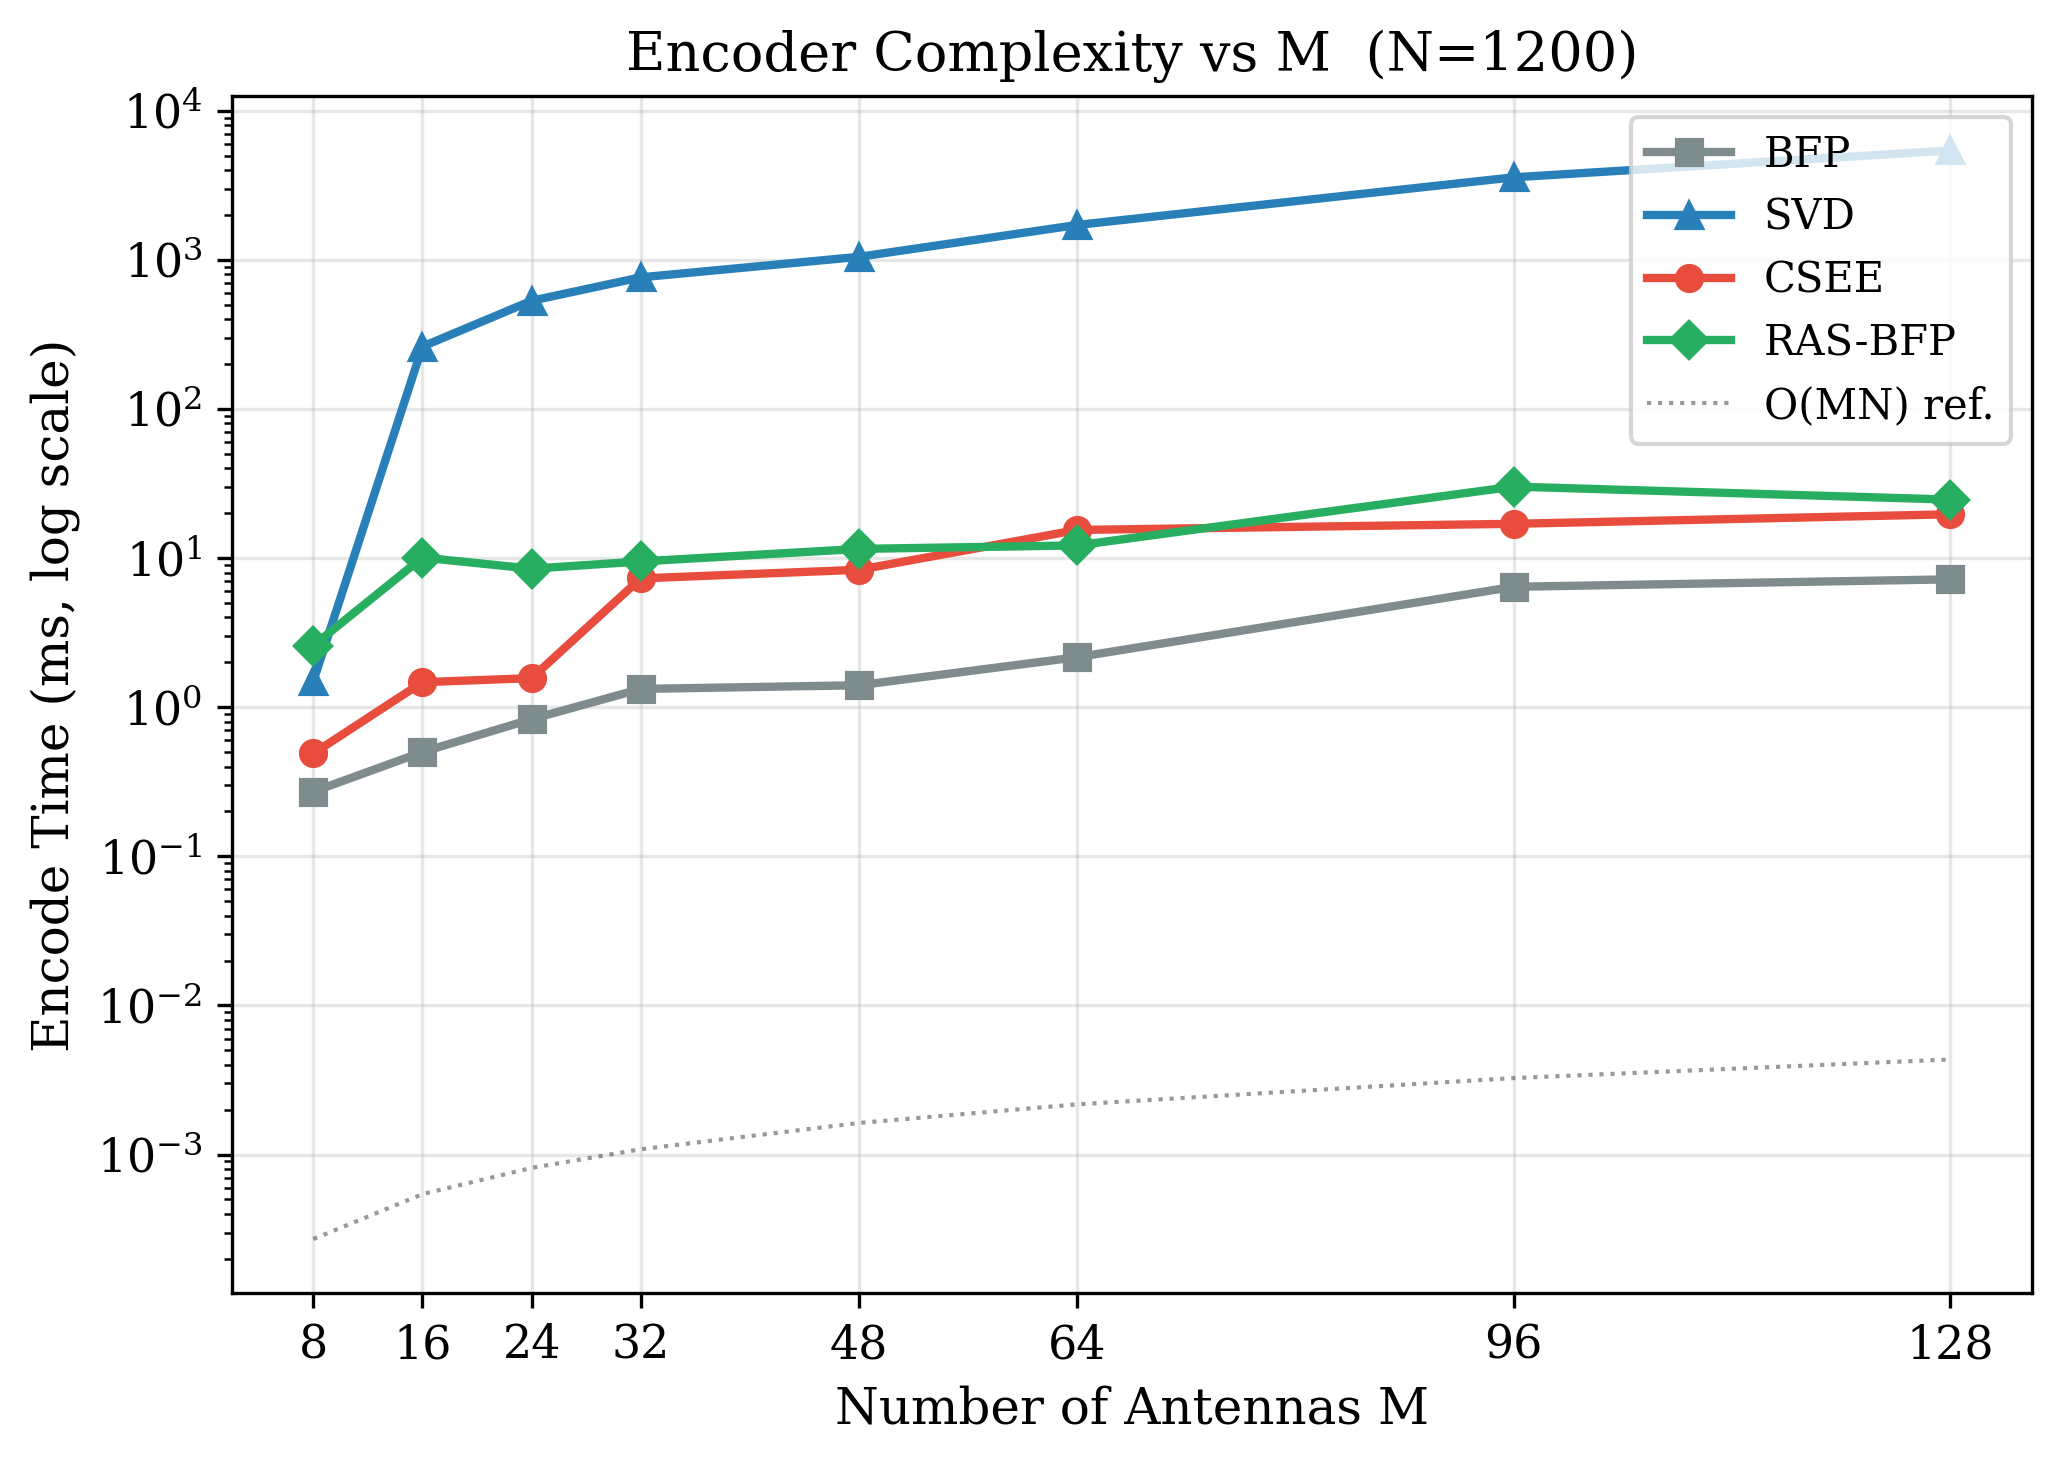
\includegraphics[width=\linewidth]{exp2_complexity.png}
\caption{Encode time versus array size.}
\label{fig:exp2}
\end{subfigure}\hfill
\begin{subfigure}{0.49\textwidth}
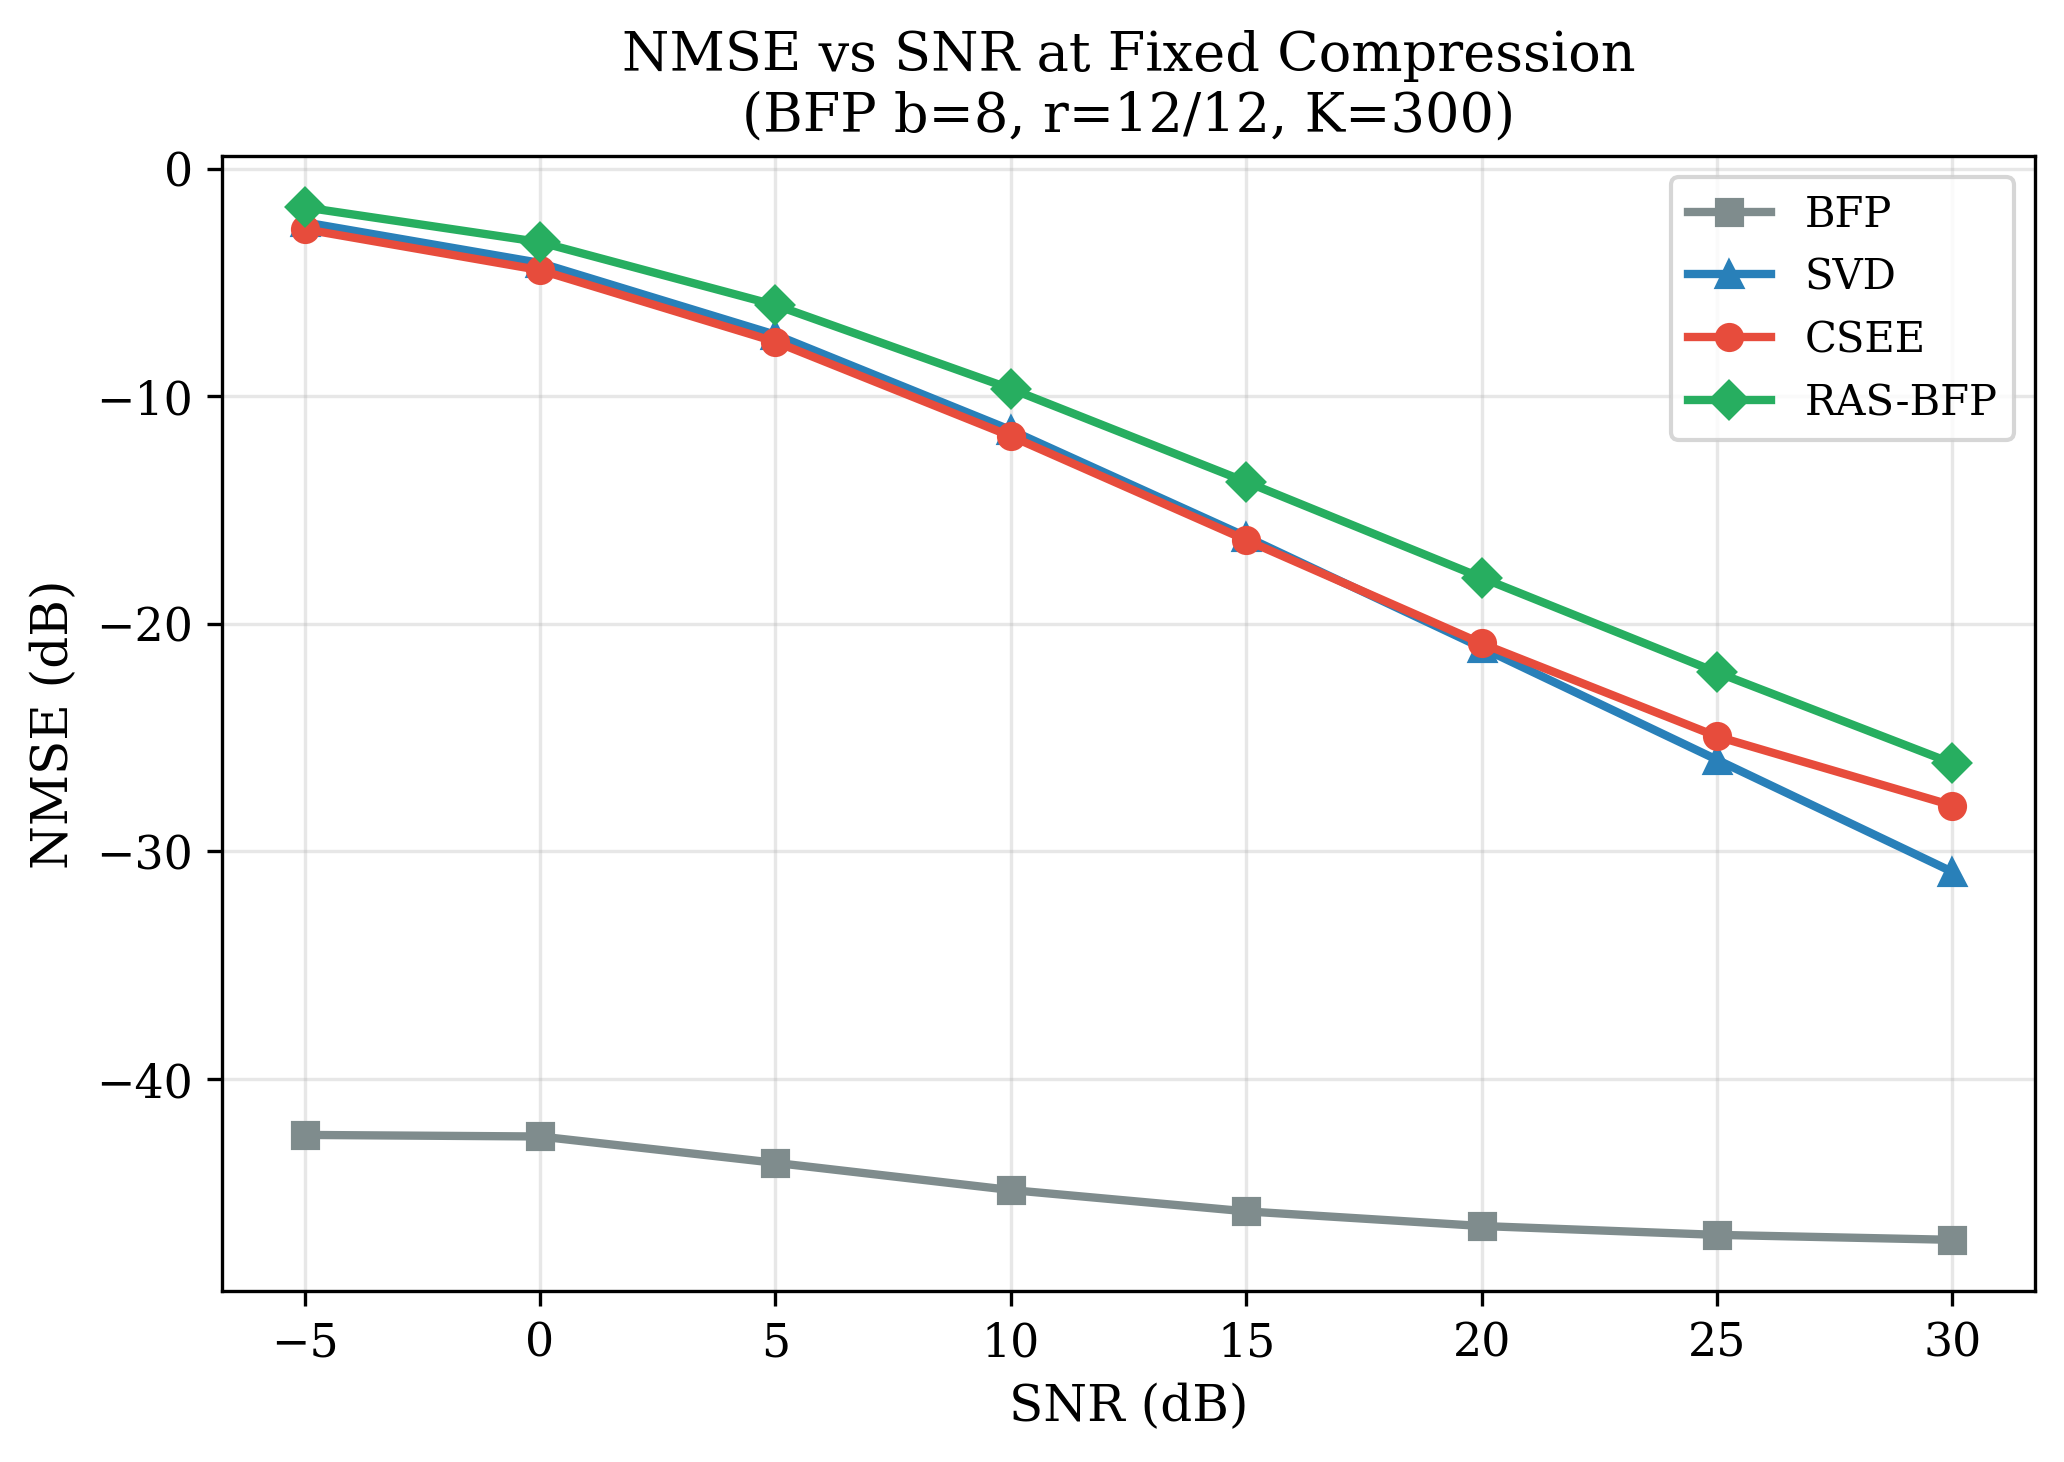
\includegraphics[width=\linewidth]{exp4_snr_sweep.png}
\caption{NMSE versus SNR.}
\label{fig:exp4}
\end{subfigure}
\caption{Complexity and SNR robustness of the encoders: the proposed methods scale near-linearly and keep their accuracy across SNR.}
\end{figure}

\section{Matrix-Inversion Benchmark Results}
\label{sec:ra-bench}

Table~\ref{tab:a-bench} lists the mean and 95th-percentile latency on the held-out matrices of size $n = 100$. Every method is timed through the same Python call path, one matrix per call, so per-call overhead is part of every number and the table ranks methods as they would be used from a Python control loop. In this setting InverseNet-Ultra has the lowest mean latency of the eight methods (0.47~ms) and a 2$\times$ lower 95th percentile than LAPACK (0.57 vs 1.13~ms). It is 2.7$\times$ faster than classical Newton--Schulz and 7$\times$ faster than LU (scipy). The main outcome of the screening is the choice of method family: a Newton--Schulz iteration with a good initial guess, which RMT-WS develops for the complex precoding workload below and Chapter~\ref{ch:impl} implements in C.

\begin{table}[H]
\caption{Inversion screening benchmark on held-out real matrices $A = G/\sqrt n + 2I$, $n = 100$ (CPU, Python, one matrix per call).}
\label{tab:a-bench}
\centering
\begin{tabular}{lcc}
\toprule
Method & Mean & p95 \\
\midrule
\ours \textbf{InverseNet-Ultra (ours)} & \textbf{0.47~ms} & \textbf{0.57~ms} \\
LAPACK \texttt{getri} (numpy) & 0.57~ms & 1.13~ms \\
\ours InverseNet-NS (ours) & 0.97~ms & 1.06~ms \\
Newton--Schulz & 1.27~ms & 1.71~ms \\
Gauss--Jordan & 1.97~ms & 3.40~ms \\
LU (scipy) & 3.36~ms & 6.09~ms \\
SVD & 10.2~ms & 20.8~ms \\
QR & 20.3~ms & 64.5~ms \\
\bottomrule
\end{tabular}
\end{table}

The learned iteration works because it keeps the Newton--Schulz structure and learns only its coefficients: it needs a handful of parameters, generalises across matrices, and a fixed number of batched matrix multiplications gives a flat, predictable latency. This principle, \emph{keep the mathematical structure and learn only what is uncertain}, leads directly to RMT-WS and, in Part~B, to the KKT newsvendor rule.

\section{RMT-WS Results on Complex Precoding Channels}
\label{sec:ra-rmtws}

\subsection{Spectral interval}

Figure~\ref{fig:mp}(a) confirms that the spectrum of the equilibrated Gram matrix follows the Marchenko--Pastur law for i.i.d.\ channels. Table~\ref{tab:a-interval} and Figure~\ref{fig:mp}(b) compare how often the interval $[a,b]$ contains the true spectrum. Our moment-matched interval covers the upper edge in 100\,\% of cases on every channel type and gives 2$\times$ better lower-edge coverage than the classical fixed-ratio bound on strongly correlated and line-of-sight channels, with only $K^2$ work.

\begin{table}[H]
\caption{Probability that $[a,b]$ contains the true spectrum (24 subcarriers $\times$ 30 drops).}
\label{tab:a-interval}
\centering\small
\begin{tabular}{lcc|cc}
\toprule
& \multicolumn{2}{c|}{Fixed-ratio MP + Weyl} & \multicolumn{2}{c}{\textbf{Moment-matched MP (ours)}} \\
Channel & lower edge & upper edge & lower edge & upper edge \\
\midrule
i.i.d., equal gain & 98.9\,\% & 99.3\,\% & \textbf{100\,\%} & \textbf{100\,\%} \\
UMa near-far & 99.6\,\% & 99.9\,\% & \textbf{100\,\%} & \textbf{100\,\%} \\
12$^\circ$ angular spread + near-far & 96.8\,\% & 99.4\,\% & \textbf{100\,\%} & \textbf{100\,\%} \\
3$^\circ$ angular spread + near-far & 61.1\,\% & 94.7\,\% & \textbf{90.6\,\%} & \textbf{100\,\%} \\
Rician 6~dB + 12$^\circ$ & 41.3\,\% & 90.7\,\% & \textbf{84.0\,\%} & \textbf{100\,\%} \\
\bottomrule
\end{tabular}
\end{table}

\begin{figure}[H]
\centering
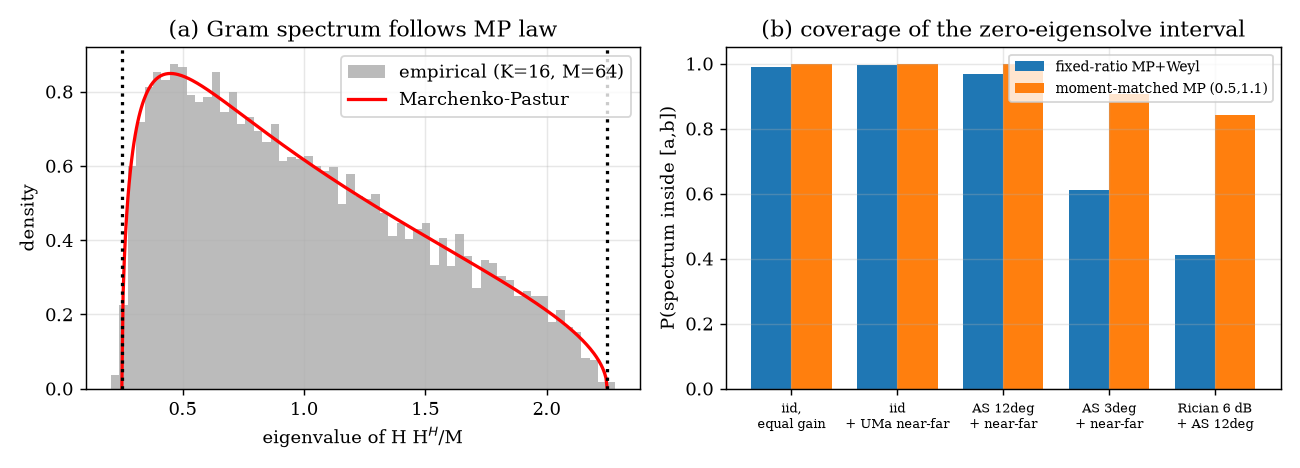
\includegraphics[width=\textwidth]{exp5_spectrum_probability.png}
\caption{(a) The Gram spectrum follows the Marchenko--Pastur law; (b) coverage of the eigensolve-free interval: the moment-matched interval (orange) adapts to correlation and line-of-sight where the fixed-ratio bound (blue) fails.}
\label{fig:mp}
\end{figure}

\subsection{Cold-start inversion cost}

Table~\ref{tab:a-cold} counts the complex GEMMs ($K^3$ multiply-accumulates each) needed to reach at most 1\,\% RZF sum-rate loss. The Chebyshev--MP initialisation followed by Newton--Schulz converges in 6 GEMMs where Neumann-type and classical Newton schemes need more than 10, beats every Neumann/Newton-type scheme, and is the best of all methods at heavy load ($K/M = 0.5$: 9 versus 12 GEMMs).

\begin{table}[H]
\caption{Complex GEMMs needed for $\le 1\,\%$ sum-rate loss (cold start), configurations $M/K$.}
\label{tab:a-cold}
\centering
\begin{tabular}{lcc}
\toprule
Method & 64/16 & 64/32 \\
\midrule
Neumann series (Wu / Prabhu~\cite{wu2013,prabhu2013}) & $>8$ & $>8$ \\
Joint Newton--Neumann (Shao~\cite{shao2016}) & $>10$ & $>10$ \\
Newton--Schulz, classical initialisation & $>10$ & $>10$ \\
Block conjugate gradient & 7 & 12 \\
Gauss--Seidel & 6 & $>12$ \\
\ours \textbf{Chebyshev-MP + Newton--Schulz (ours)} & \textbf{6} & \textbf{9} \\
\bottomrule
\end{tabular}
\end{table}


\subsection{Warm-start tracking across user speeds}

Table~\ref{tab:a-track} and Figure~\ref{fig:exp7} compare RMT-WS with warm-started Gauss--Seidel and conjugate gradient at 3, 30 and 120~km/h ($K=16$, $M=64$). At pedestrian speed RMT-WS needs 2.7$\times$ fewer GEMMs than a cold start at 30$\times$ lower loss; at 30~km/h it has the lowest loss of all warm-started methods; at 120~km/h it has 24$\times$ lower loss than warm Gauss--Seidel. Fixed one- or two-step warm starts diverge at 120~km/h, whereas the certificate makes RMT-WS fall back to a cold start and never diverge: one method serves every speed. It is cheap when users are slow and safe when they are fast.

\begin{table}[H]
\caption{Tracking: sum-rate loss versus exact RZF / GEMMs per slot per PRB ($K=16$, $M=64$).}
\label{tab:a-track}
\centering
\begin{tabular}{lccc}
\toprule
Speed & Warm Gauss--Seidel $\times 4$ & Warm CG $\times 4$ & \textbf{RMT-WS (ours)} \\
\midrule
3~km/h & 0.009\,\% / 4 & 0.013\,\% / 5 & \textbf{0.006\,\% / 2.25} \\
30~km/h & 0.63\,\% / 4 & 0.96\,\% / 5 & \textbf{0.43\,\% / 5.2} \\
120~km/h & 2.9\,\% / 4 & 5.5\,\% / 5 & \textbf{0.12\,\% / 6.25} \\
\bottomrule
\end{tabular}
\end{table}

\begin{figure}[H]
\centering
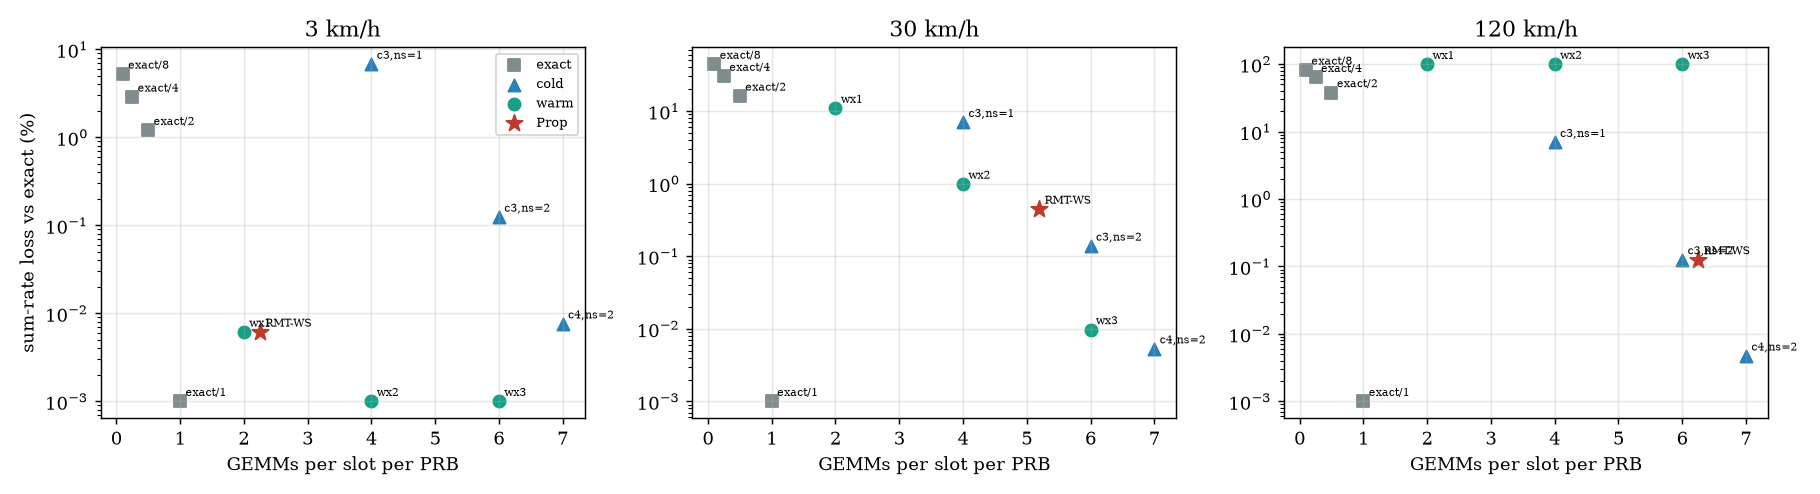
\includegraphics[width=\textwidth]{exp7_tracking.png}
\caption{Tracking accuracy versus cost at 3, 30 and 120~km/h; RMT-WS (red star) sits at the low-cost, low-loss corner at every speed.}
\label{fig:exp7}
\end{figure}

\subsection{Doppler law and certificate}

Figure~\ref{fig:exp12} validates the Doppler-to-warm-start law of Eq.~\eqref{eq:doppler}: the measured initial residual grows linearly with user speed (log-log slope 1.00), and the predicted number of Newton steps matches the measurement. The law gives the DU an explicit warm-start envelope (39~km/h for $M=64$, $K=16$). In an audit of 480 PRB cases from 3 to 120~km/h, zero warm starts accepted by the certificate at $\hat r \le 0.3$ were non-contractive.

\begin{figure}[H]
\centering
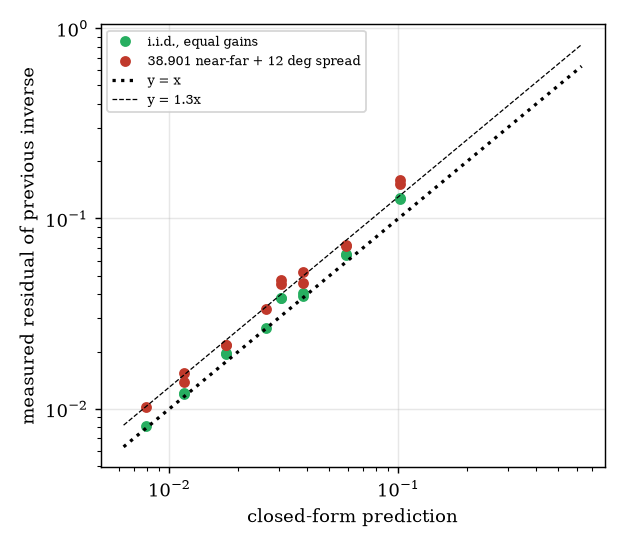
\includegraphics[width=0.62\textwidth]{exp12_doppler_law.png}
\caption{Doppler-to-warm-start law: the initial residual grows linearly with user speed, as predicted.}
\label{fig:exp12}
\end{figure}

\subsection{Robustness at low precision}

Accelerators such as tensor cores and NPUs compute GEMMs with low-precision operands and wide accumulation. Table~\ref{tab:a-lowprec} and Figure~\ref{fig:exp8} show that our Chebyshev + 3 Newton--Schulz inversion keeps 6$\times$ lower loss than direct Gauss--Jordan inversion at 8 mantissa bits and 3.6$\times$ lower at 6 bits, because each Newton step corrects the rounding error of the previous one. The tracker at 8 bits loses only 0.70\,\% against 0.54\,\% at full precision at 30~km/h. RMT-WS is therefore ready for low-precision accelerators where direct inversion degrades.

\begin{table}[H]
\caption{Sum-rate loss versus float64 exact inversion at low precision.}
\label{tab:a-lowprec}
\centering
\begin{tabular}{lcc}
\toprule
Setting & Direct Gauss--Jordan & \textbf{Ours (Chebyshev + 3 NS)} \\
\midrule
8 mantissa bits & 0.88\,\% & \textbf{0.15\,\%} \\
6 mantissa bits & 5.1\,\% & \textbf{1.4\,\%} \\
Ill-conditioned, 10 bits & 1.2\,\% & \textbf{0.49\,\%} \\
\bottomrule
\end{tabular}
\end{table}

\begin{figure}[H]
\centering
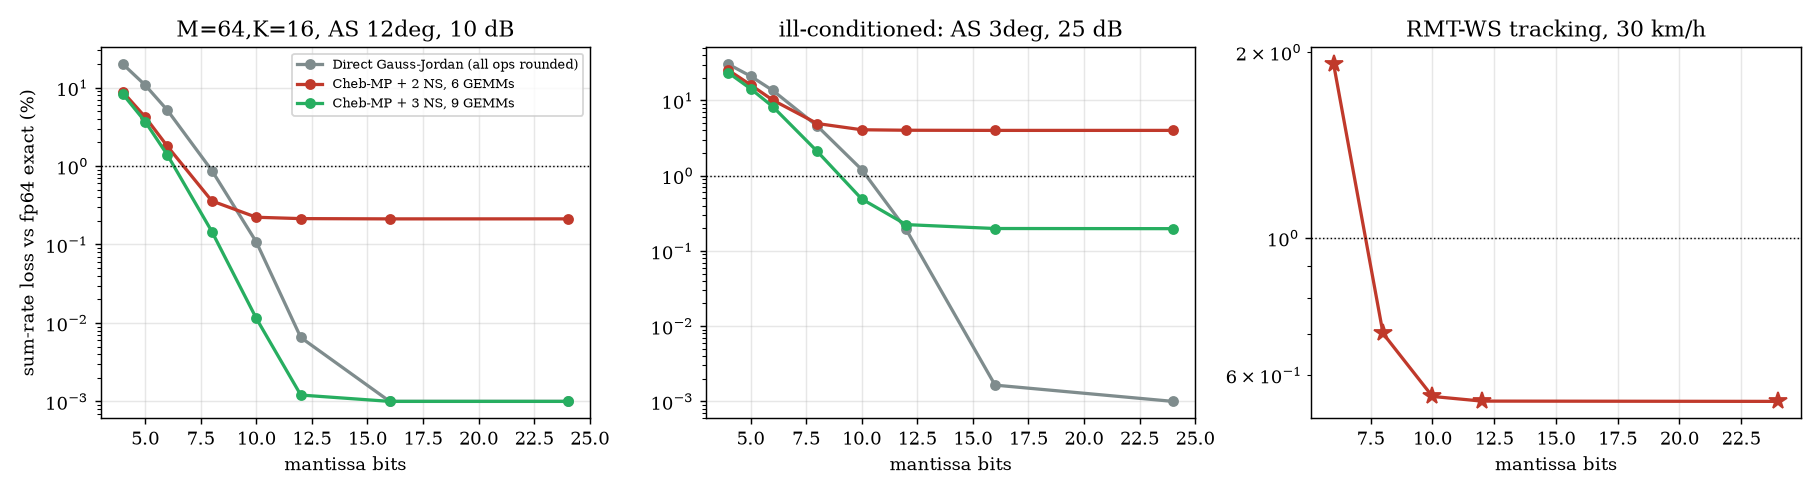
\includegraphics[width=0.85\textwidth]{exp8_low_precision.png}
\caption{Sum-rate loss versus mantissa bits: Newton refinement keeps the loss low where direct inversion degrades.}
\label{fig:exp8}
\end{figure}

\subsection{Comparison with existing complex-inversion methods}

Table~\ref{tab:a-vs-sota} collects the head-to-head comparisons. On every compared metric RMT-WS and its fused kernel are better than the listed existing method.

\begin{table}[H]
\caption{RMT-WS against existing complex-inversion methods.}
\label{tab:a-vs-sota}
\centering\small
\renewcommand{\arraystretch}{1.12}
\begin{tabularx}{\textwidth}{>{\raggedright\arraybackslash}X>{\raggedright\arraybackslash}p{3.6cm}cc}
\toprule
Existing method & Metric & Existing & \textbf{RMT-WS (ours)} \\
\midrule
Neumann series~\cite{wu2013,prabhu2013} & GEMMs for $\le 1\,\%$ loss & $>8$ & \textbf{6} \\
Joint Newton--Neumann~\cite{shao2016} & GEMMs for $\le 1\,\%$ loss & $>10$ & \textbf{6} \\
Newton--Schulz, classical init.~\cite{benisrael1966,pan1991} & GEMMs for $\le 1\,\%$ loss & $>10$ & \textbf{6} \\
Gauss--Seidel & GEMMs, $K/M = 0.5$ & $>12$ & \textbf{9} \\
Block conjugate gradient & GEMMs, $K/M = 0.5$ & 12 & \textbf{9} \\
Warm-started Gauss--Seidel $\times 4$ & loss at 120~km/h & 2.9\,\% & \textbf{0.12\,\%} \\
Warm-started CG $\times 4$ & loss at 30 / 120~km/h & 0.96 / 5.5\,\% & \textbf{0.43 / 0.12\,\%} \\
Fixed 1-/2-step warm start & loss at 120~km/h & diverges & \textbf{0.13\,\%} \\
Direct Gauss--Jordan, 8-bit & sum-rate loss & 0.88\,\% & \textbf{0.15\,\%} \\
Classical MP + Weyl interval & lower-edge coverage, Rician & 41\,\% & \textbf{84\,\%} \\
numpy + LAPACK (whole precoder) & time per slot, $K=16$ & 3.21~ms & \textbf{0.226~ms} \\
\bottomrule
\end{tabularx}
\end{table}

\section{Fronthaul Impact of RU-Side Precoding}
\label{sec:ra-ru}

Table~\ref{tab:a-ru} and Figure~\ref{fig:exp10} quantify the architectures of Figure~\ref{fig:ru-prec} for a 100~MHz carrier with $M=64$, $K=16$ and BFP-9 IQ. Precoding at the radio unit with 8-bit weights refreshed every slot cuts the fronthaul from 118.4 to 32.8~Gbit/s ($-72\,\%$, 3.6$\times$ lighter) at 99.7\,\% of the exact RZF sum-rate. Refreshing the weights less often is not an option at mobility (every 4 slots gives only 70\,\% of the rate at 30~km/h), so per-slot weights are required, and this is exactly the workload our fast precoder handles.

\begin{table}[H]
\caption{Fronthaul rate and sum-rate by precoding architecture (100~MHz, $M=64$, $K=16$, BFP-9).}
\label{tab:a-ru}
\centering
\begin{tabular}{lcc}
\toprule
Architecture & Fronthaul & Sum-rate vs exact \\
\midrule
DU precodes, sends 64 streams & 118.4~Gbit/s & 100\,\% \\
\ours \textbf{RU precodes, 16 layers + 8-bit weights} & \textbf{32.8~Gbit/s ($-72\,\%$)} & \textbf{99.7\,\%} \\
RU precodes, 16 layers + 6-bit weights & 32.0~Gbit/s ($-73\,\%$) & 96.7\,\% \\
\bottomrule
\end{tabular}
\end{table}

\begin{figure}[H]
\centering
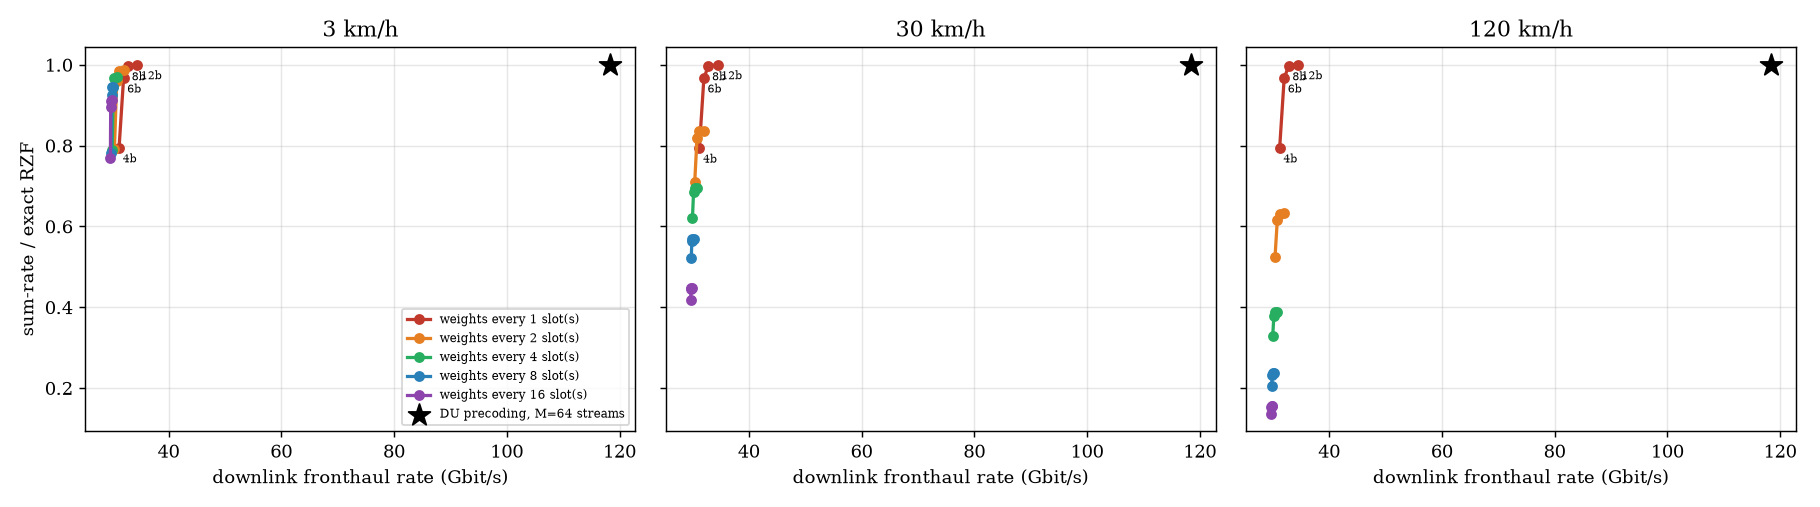
\includegraphics[width=0.9\textwidth]{exp10_fronthaul.png}
\caption{Fronthaul rate and sum-rate by precoding architecture and weight refresh period.}
\label{fig:exp10}
\end{figure}

\section{Summary}

This chapter presented the simulation results of Part~A. The structure-aware encoders compress reference-symbol and channel IQ 6.4--8.1$\times$ against 16-bit I/Q (32$\times$ at the CSEE knee), 3--4 times the ratio of the O-RAN standard, and run 3--6$\times$ faster than SVD. The inversion screening selected a learned Newton--Schulz family, with the lowest mean and a 2$\times$ lower tail latency than LAPACK at $n = 100$. RMT-WS inverts realistic complex Grams in 6 GEMMs instead of more than 10, tracks users at every speed with a certificate that never accepted an unsafe step, and is robust at 8-bit precision. Together with the fused kernel of Chapter~\ref{ch:impl} it enables RU-side precoding with a 72\,\% lighter fronthaul at 99.7\,\% of the exact sum-rate.
